\section{Generation d'une Suite de \textit{Chirps}}

Il est possible de répéter la génération d'un \textit{chirp} $K$ fois en utilisant l'équation \ref{eq:t_all_chirps} comme base de temps afin d'obtenir une suite de \textit{chirps} qui va composer le signal qui sera envoyé.

\begin{equation}
    t = kT + t^\prime
    \label{eq:t_all_chirps}
\end{equation}

 Avec $t^\prime$ qui est le temps par \textit{chirp} (\(t^\prime \in [0,T]\)) et k qui est le \textit{chirp} qui est généré (\(k \in [0,K-1]\)). Dans la simulation, le paramètre $K$ vaut 256.

\section{Simulation des \textit{Chirps} Reçues}

Après avoir été émis, le signal va être réfléchis par les cibles et revenir avec un certain décalage temporel du à la distance et fréquentiel du à la vitesse de la cible. Dix cibles aléatoires ont été simulées dans le code fournit avec ce laboratoire. La figure \ref{fig:all_chirp} montre le signal qui est émis et les signaux qui sont réfléchis par les différentes cibles. Étant donné le fait que les cibles sont dans la voisinage du radar, les signaux réfléchis sont très proches des signaux émis. La figure \ref{fig:all_chirp_zoom} est un agrandissement de la figure \ref{fig:all_chirp} qui permet de distinguer les différents signaux réfléchis. 

\begin{figure}[H]
  \centering
  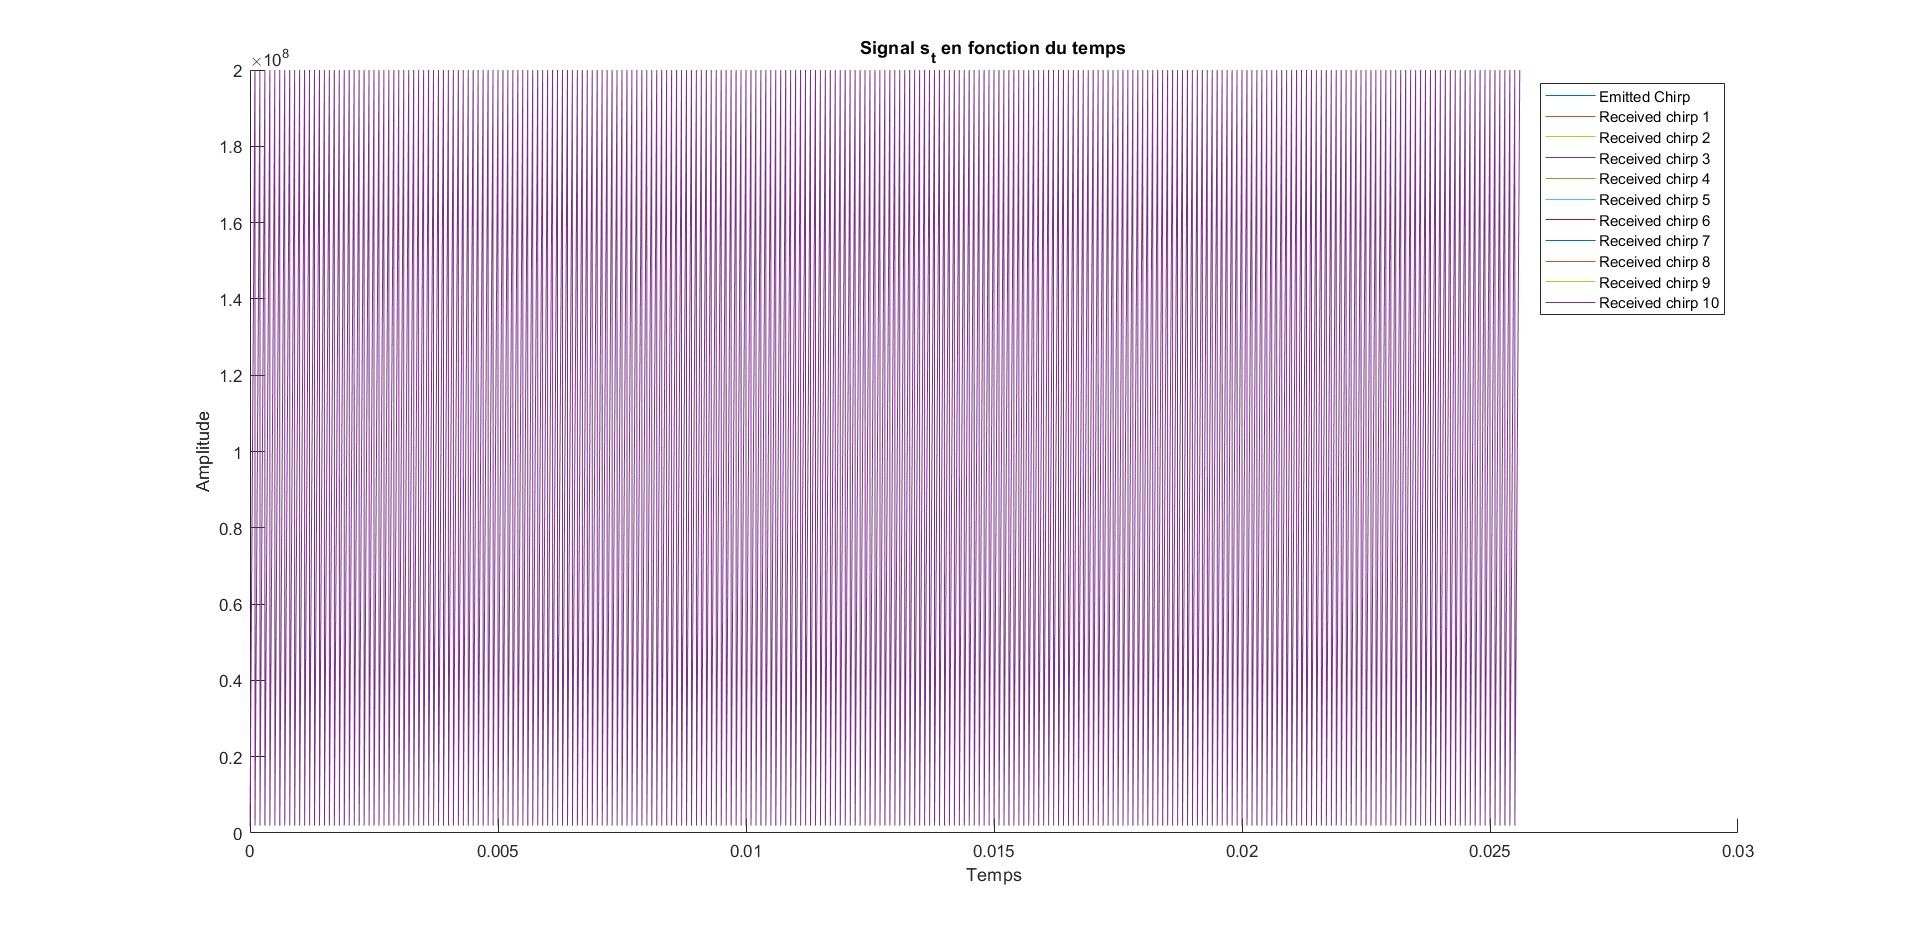
\includegraphics[scale = 0.2]{Pictures/multiple_target.jpg}  \caption{Vue d'ensemble des \textit{chirps} émis et reçus}
  \label{fig:all_chirp}
\end{figure}

\begin{figure}[H]
  \centering
  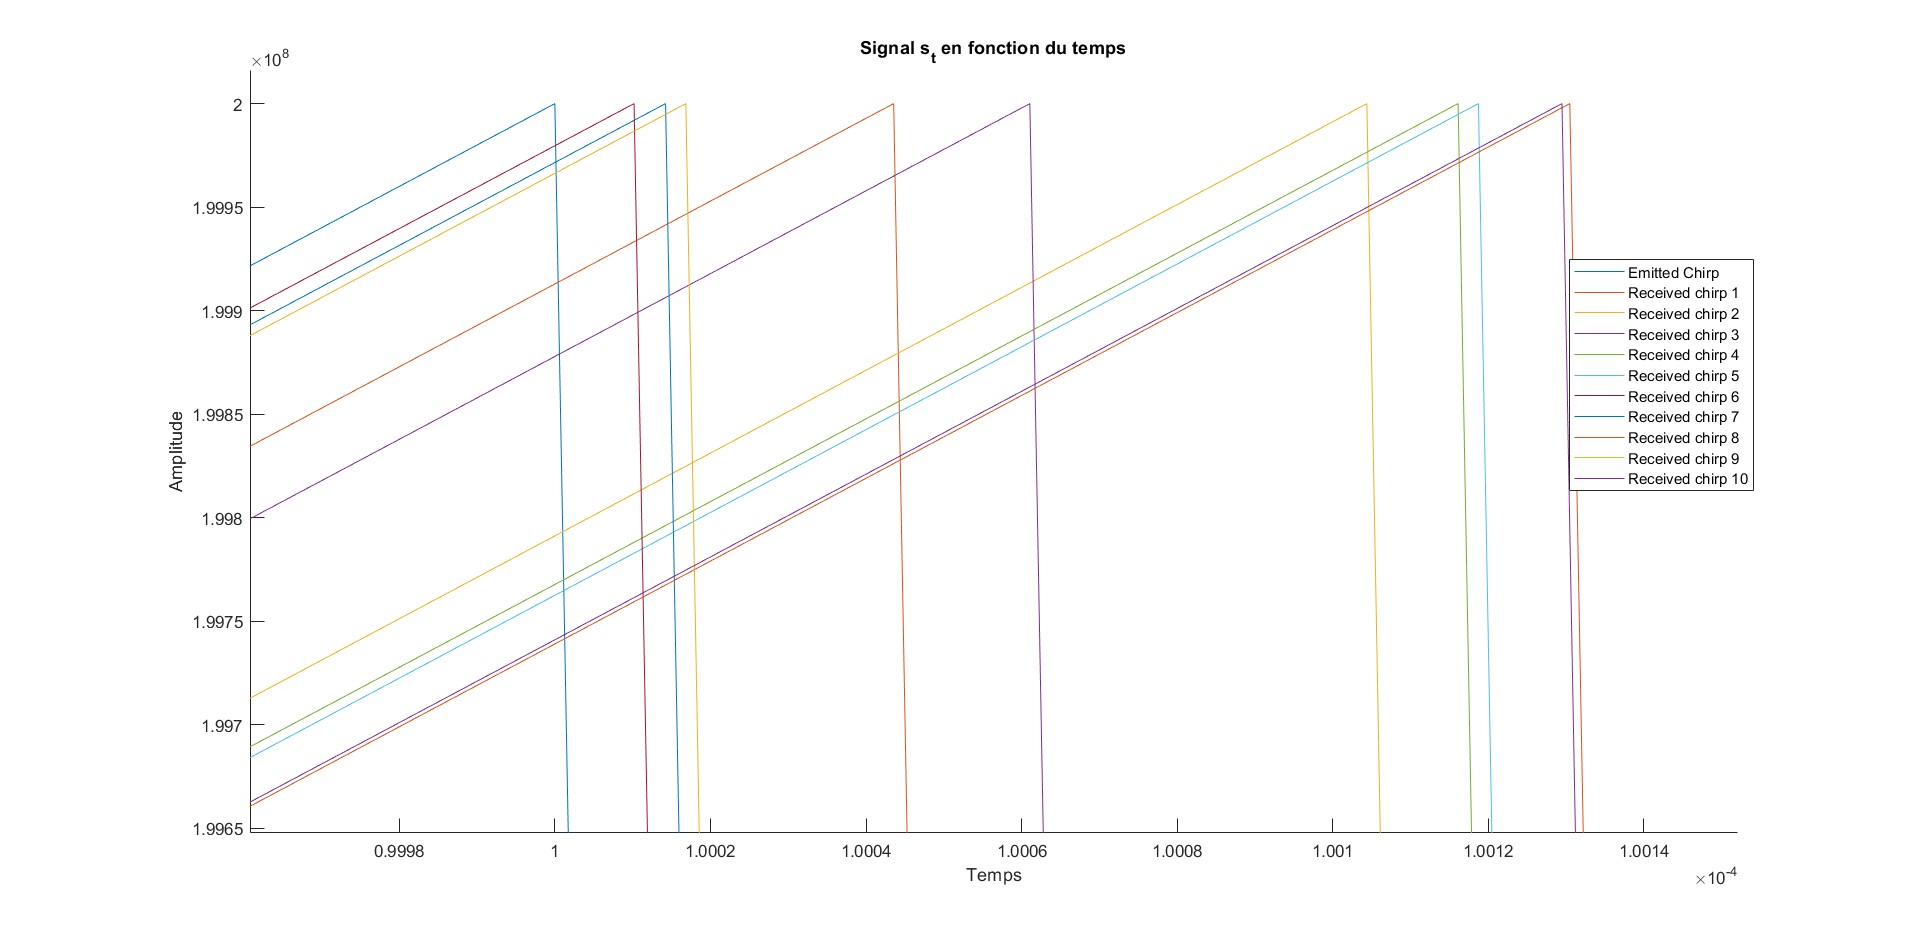
\includegraphics[scale = 0.2]{Pictures/multiple_target_zoom.jpg}  \caption{Vue rapprochée des \textit{chirps} émis et reçus}
  \label{fig:all_chirp_zoom}
\end{figure}

